\chapter{Theoretischer Hintergrund}
\section{E-Learning und digitale Wissensvermittlung}
E-Learning stellt eine moderne Lernumgebung dar, die durch den Einsatz von digitalen Medien und Technologien die Wissensvermittlung unterstützt.
Sie hat sich in den 1990er Jahren entwickelt und ermöglicht den Lernenden, unabhängig von Zeit und Ort zu lernen sowie die Integration einer Vielzahl von Lernmaterialien und -methoden.
Durch den Einsatz von E-Learning können Lernende ihr Wissen effizienter und flexibler erweitern und vertiefen.
Dieser Ansatz hat in den letzten Jahren an Bedeutung gewonnen und wird zunehmend in Bildungseinrichtungen und Unternehmen eingesetzt.
So fördert E-Learning die Selbstorganisation, kritisches Denken und die Fähigkeit zur Problemlösung der Lernenden.
\footcite[Vgl.][S. 203 f.]{jethroELearningItsEffects2012}
Zudem ermöglicht E-Learning eine individuelle Anpassung des Lernprozesses an die Bedürfnisse und Präferenzen der Lernenden.

Der Begriff „E-Learning“ umfasst verschiedene Formen des elektronisch unterstützten Lernens, worunter bspw. Online-Kurse, Webinare, virtuelle Klassenzimmer und interaktive Lernplattformen fallen.
Diese Methoden bieten eine interaktive und dynamische Lernumgebung, die traditionelle Lehrmethoden ergänzt und in vielen Fällen ersetzt.
Eine der größten Stärken des E-Learnings liegt in seiner Flexibilität: Lernende können in ihrem eigenen Tempo arbeiten und auf eine Vielzahl von Ressourcen zugreifen, die von Texten und Videos bis hin zu interaktiven Simulationen reichen.
Ein weiterer wesentlicher Vorteil des E-Learnings ist die Möglichkeit der kontinuierlichen Aktualisierung und Erweiterung von Lerninhalten. 

Durch den Einsatz von \acp{LMS} können Bildungsanbieter Inhalte schnell und effizient aktualisieren und an neue wissenschaftliche Erkenntnisse oder technologische Entwicklungen anpassen.
\footcite[Vgl.][22]{nedevaADVANTAGESELEARNINGENGLISH2010}
Diese Systeme ermöglichen es auch, den Lernfortschritt zu überwachen und gezielte Unterstützung anzubieten, was zu einer effektiveren Lernkontrolle und -steuerung führt.
\footcite[Vgl.][1]{zhangMoodogTrackingStudents2007}
E-Learning bietet zudem die Möglichkeit der Vernetzung und Zusammenarbeit zwischen Lernenden.
Durch Foren, Chats und Videokonferenzen können Lernende miteinander in Kontakt treten, sich austauschen und gemeinsam an Projekten arbeiten.
Diese sozialen Interaktionen fördern nicht nur das Lernen, sondern auch wichtige soziale Kompetenzen und Teamfähigkeit.
Ein weiterer Aspekt der digitalen Wissensvermittlung ist die Möglichkeit der Personalisierung.
Adaptive Lernsysteme passen sich den individuellen Bedürfnissen und Lernstilen der Lernenden an, indem sie deren Fortschritte analysieren und darauf basierend maßgeschneiderte Lernwege vorschlagen. Diese personalisierte Herangehensweise maximiert die Effizienz des Lernprozesses und stellt sicher, dass die Lernenden die für sie relevanten Inhalte in der optimalen Reihenfolge und Tiefe bearbeiten können.

Zusammenfassend lässt sich sagen, dass E-Learning und digitale Wissensvermittlung eine bedeutende Transformation im Bildungswesen darstellen.
Sie bieten flexible, effiziente und personalisierte Lernmöglichkeiten, die den Lernenden helfen, ihre Ziele effektiver zu erreichen.
Durch die kontinuierliche Weiterentwicklung und Integration neuer Technologien wird E-Learning auch in Zukunft eine zentrale Rolle in der Bildung spielen und zur Verbesserung der Lernprozesse und Lernergebnisse beitragen.

E-Learning stellt eine neue Lernumgebung dar, die durch den Einsatz von digitalen Medien und 
Technologien die Wissensvermittlung unterstützt. Es ermöglicht den Lernenden, unabhängig von Zeit und 
Ort zu lernen und bietet eine Vielzahl von Lernmaterialien und -methoden.
\footcite[Vgl.][1]{hosseindoostShiftTraditionalLearning2022}
Durch den Einsatz von E-Learning können Lernende ihr Wissen effizienter und flexibler erweitern und vertiefen.
Dieser Ansatz hat in den letzten Jahren an Bedeutung gewonnen und wird zunehmend in 
Bildungseinrichtungen und Unternehmen eingesetzt.
So fördert E-Learning die Selbstorganisation, kritisches
Denken oder die Fähigkeit zur Problemlösung der Lernenden. 

\section{Didaktische Konzepte für die Wissensquiz-Erstellung}
Die Erstellung von Wissensquizzen erfordert eine sorgfältige Planung und Umsetzung, um die Lernziele effektiv zu erreichen.
Dabei spielen verschiedene didaktische Konzepte eine wichtige Rolle, um sicherzustellen, dass die Quizfragen relevant, anspruchsvoll und motivierend sind.
Für die Gestaltung von Schulungsartefakten
hat sich in der Wissenschaft mit dem „\ac{ADDIE}“-Modell ein strukturiertes
Vorgehensmodell etabliert, welches den gesamten Entwicklungsprozess von der Analyse über das Design und die Implementierung bis hin zur Evaluation umfasst.
Aus diesem Grund wird im Folgenden das \ac{ADDIE}-Modell vorgestellt und erläutert, wie es für die Erstellung von Wissensquizzen eingesetzt werden kann (siehe Abb. \ref{fig:mondrian}).
\footcite[Vgl.][1805]{nadiyahDevelopmentOnlineProject2015}
\begin{figure}[H]
    \centering
    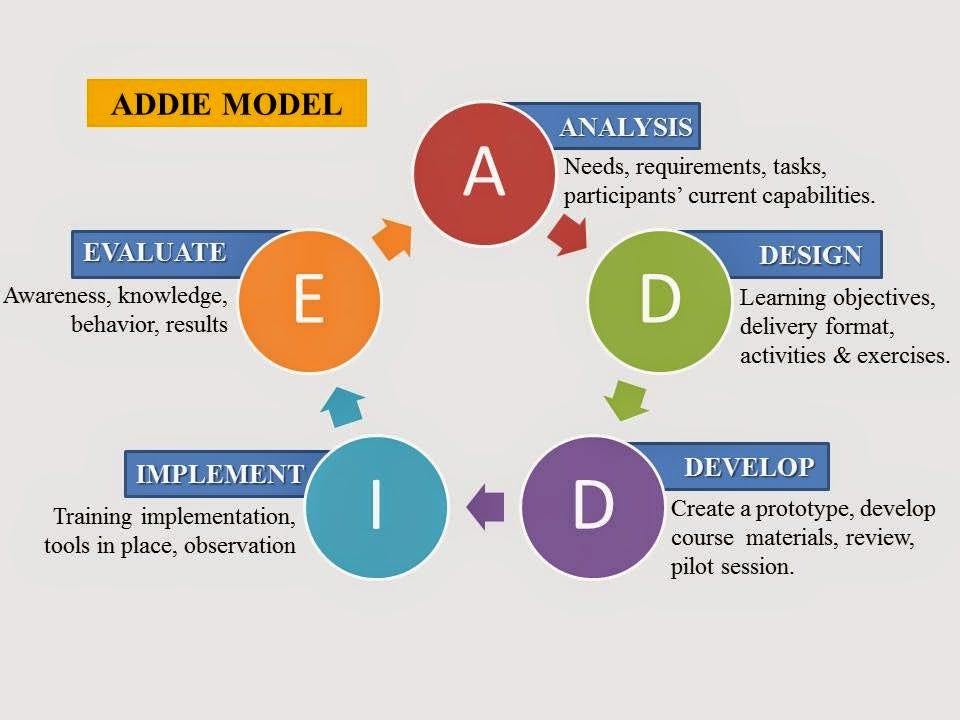
\includegraphics[width=1.0\linewidth]{graphics/addie_model.jpg}
    \caption[Das \acs{ADDIE}-Modell im Überblick.]{Das \ac{ADDIE}-Modell im Überblick.\protect\footnotemark}
    \label{fig:mondrian}
\end{figure}
\footnotetext{Enthalten in: \cite[352]{kuzminskaIVEFFECTIVEMETHODS2017}}
Die erste Phase im \ac{ADDIE}-Modell sieht die Durchführung einer Bedarfsanalyse vor, um die Lernziele und -bedürfnisse der Zielgruppe korrekt erfassen zu können.
Als Möglichkeit hierfür wird von Allen 2006 unter anderem die Erstellung einer Aufgabenliste vorgeschlagen, welche für
den Vergleich mit den Fähigkeiten und Kenntnissen der Zielgruppe genutzt werden kann.
\footcite[Vgl.][436]{allenOverviewEvolutionADDIE2006}
Hierbei ist ein besonderes Augemerk auf die Unterschiede zwischen dem gegenwärtigen Ist- und dem gewünschten Soll-Zustand in Bezug auf das vorhandene Wissen zu legen.
\footcite[Vgl.][436]{allenOverviewEvolutionADDIE2006}
Auf dieser Basis können schließlich Anforderungen an das zu erstellende Schulungsartefakt abgeleitet werden.
Für den vorliegenden Anwendungsfall der Quizerstellung in Moodle bedeutet dies, dass die Sekretärinnen und Sekretären
der Fakultät als Zielgruppe zu identifizieren sind und daher die Fragen entsprechend deren Kenntnisstand und Bedürfnissen gestaltet werden müssen.
So ist bspw. von Fragen, welche bloße Fakten und Definitionen abfragen, ebenso abzusehen wie von Fragen, welche
primär IT-administratives Fachwissen erfordern. Eine Zusammensetzung von Fragen, welche
einerseits theoretischer Natur sind und andererseits auch praktische Anwendungsfälle abbilden, scheint hingegen sinnvoll.
Letzteres könnte bspw. durch die Einbindung von Fallbeispielen oder Praxisübungen erfolgen, während für den
theoretischen Teil komplexere Fragen, welche ein tieferes Verständnis von Rapla erfordern, genutzt werden könnten.

Den zweiten Schritt im \ac{ADDIE}-Modell bildet die Design-Phase, in welcher eine detaillierter Plan an Anweisungen und Inhalten für das zu erstellende Schulungsartefakt erstellt wird.
Hierunter fällt auch die Auswahl entsprechender Lehrmethoden und -medien sowie eine kritische Überprüfung aktuell vorliegender Materialien.
\footcite[Vgl.][436]{allenOverviewEvolutionADDIE2006} 
Gemäß xx ist in dieser Phase insbesondere darauf zu achten, dass anhand des aufgestellten Plans letztlich eine präzise Abbildung der festgelegten Ziele erfolgt.
Ebenfalls Gegenstand dieser Phase ist die Entwicklung konzeptioneller Grundlagen für das zu erstellende Artefakt, worunter
bspw. die Entwicklung oder die Implementierung eines geeigneten Bildungsinformationsmanagementsystems fallen könnte.
\footcite[Vgl.][436]{allenOverviewEvolutionADDIE2006}
Von besonderer Relevanz
ist in dieser Phase auch die Taxonomie nach Bloom, die eine Klassifizierung von Lernzielen und -aktivitäten ermöglicht.
\dots

In der dritten Phase des \ac{ADDIE}-Modells erfolgt die Implementierung des eigentlichen Schulungsartefakts.
Für den vorliegenden Anwendungsfall fällt hierunter die tatsächliche Erstellung des Wissensquiz in Moodle.
Als alternative Entwicklungsinhalte könnten laut Allen 2006 hierunter auch Videos, Simulationen oder interaktive Lernmaterialien fallen.
\footcite[Vgl.][437]{allenOverviewEvolutionADDIE2006}
Ebenso ist die Revision des erstellten Schulungsartefakts in dieser Phase von Bedeutung, um sicherzustellen, dass die erstellten Inhalte den zuvor festgelegten Anforderungen entsprechen.
\footcite[Vgl.][437]{allenOverviewEvolutionADDIE2006}

In der vierten Phase wird das erstellte Schulungsartefakt in den operativen
Betrieb überführt. Ebenso ist hierbei die Sammlung von ersten Rückmeldungen
der Nutzerinnen und Nutzer von Bedeutung, um das Artefakt ggf. nochmals
anpassen zu können bzw. eine Grundlage für die fünfte Phase des \ac{ADDIE}-Modells zu schaffen.

Die fünfte und letzte Phase des \ac{ADDIE}-Modells bildet die Evaluation des erstellten Schulungsartefakts.
Hierbei wird kritisch überprüft, ob die erstellten Inhalte mit den zuvor festgelegten Ziele übereinstimmen und das Artefakt auf die Anforderungen der Zielgruppe abgestimmt ist.
\footcite[Vgl.][437]{allenOverviewEvolutionADDIE2006}
Ebenfalls fallen unter diese Phase Überlegungen zur Effektivität der erstellten Lösung.
\footcite[Vgl.][2]{constancioExtendedADDIEModel2018}

Insgesamt wird das \ac{ADDIE}-Modell in der Forschungsliteratur als ein effektives und strukturiertes Vorgehensmodell für die Erstellung von Schulungsartefakten angesehen.
So heben bspw. Drljača u. a. 2017 das hohe Maß an Flexibilität als Vorteil hervor, da das Modell auf verschiedene Bildungs- und Trainingsbedarfe anwendbar ist.
\footcite[Vgl.][247]{drljacaADDIEModelDevelopment2017}
Als großer Kritikpunkt hingegen wird angesehen, dass vorausgesetzt wird, dass vorab bereits
alle Anforderungen bekannt sind und sich diese im Projektverlauf nicht mehr ändern.

Als Beispiele hierfür werden von Drljača u. a. 2017 sowohl
Schwierigkeiten bzgl. der Integration von guten Ideen, welche
im Projektverlauf entstehen können, als auch Probleme im Umgang
mit unerwarteten Fehlern genannt.
\footcite[Vgl.][246]{drljacaADDIEModelDevelopment2017}

\section{Zertifizierungen als Erfolgsfaktor}
\section{Gestaltung von Usability-Tests}